\section{Le train à vapeur}\label{ex:train}

Les premiers train fonctionnaient grâce à des moteurs à vapeur. 
L'énergie stockée dans l'air et 
dans le charbon était transférée au moteur à vapeur sous forme d'énergie thermique.
Le moteur convertissait ensuite l'énergie reçue en énergie de mouvement qu'il transférait à l'ensemble du train. On considère que le charbon et l'air font partie d'un seul et même  réservoir d'énergie.

\begin{questions}
	\question Quels étaient les deux réservoirs d'énergie et le convertisseur d'énergie ?
		\begin{solution}
			Les deux réservoirs d'énergie sont d'une part celui formé par l'air et le charbon et d'autre part l'ensemble du train. Le moteur est le convertisseur.
		\end{solution}
	
	\question Le moteur convertissait l'énergie qu'il recevait en une autre forme d'énergie. Laquelle ?
		\begin{solution}
			Le moteur reçoit de l'énergie thermique et la convertit en énergie de mouvement.
		\end{solution}
	
	\question Réaliser la chaine énergétique du fonctionnement de ce train. 
		\begin{solution}
			\begin{center}
				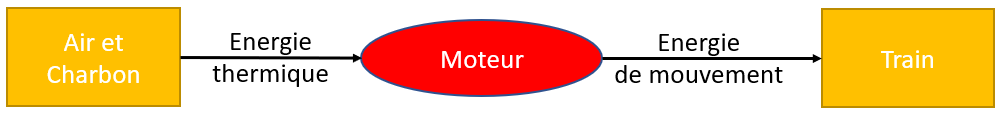
\includegraphics[scale=0.6]{img/chaine_train}
			\end{center}
		\end{solution}
		
\end{questions}